\documentclass[aspectratio=169,10pt]{beamer}

\usepackage[default]{sourcesanspro}
\usepackage{fontawesome5}
\usepackage{booktabs}
\usepackage{tabularx}
\usepackage{array}
\usepackage{tikz}
\usetikzlibrary{arrows.meta,positioning}
\usepackage{graphicx}
\usepackage[backend=biber,style=numeric,sorting=none]{biblatex}
\addbibresource{references.bib}

\definecolor{Navy}{HTML}{17324D}
\definecolor{Blue}{HTML}{247BA0}
\definecolor{Teal}{HTML}{20A39E}
\definecolor{Amber}{HTML}{E09F3E}
\definecolor{Red}{HTML}{C94C4C}
\definecolor{Ink}{HTML}{243447}
\definecolor{Muted}{HTML}{64748B}
\definecolor{Mist}{HTML}{E8EEF2}
\definecolor{Wash}{HTML}{F5F8FA}
\definecolor{PaleTeal}{HTML}{E7F7F5}
\definecolor{PaleAmber}{HTML}{FFF4E3}
\definecolor{PaleRed}{HTML}{FCECEC}

\setbeamercolor{normal text}{fg=Ink,bg=white}
\setbeamercolor{frametitle}{fg=Navy,bg=white}
\setbeamercolor{structure}{fg=Teal}
\setbeamerfont{frametitle}{size=\Large,series=\bfseries}
\setbeamertemplate{navigation symbols}{}
\setbeamersize{text margin left=0.55cm,text margin right=0.55cm}
\setbeamertemplate{frametitle}{%
  \vspace{0.20cm}\insertframetitle\par
  \vspace{-0.12cm}\color{Teal}\rule{1.05cm}{1.5pt}\color{Mist}\rule{\dimexpr\textwidth-1.05cm\relax}{1.5pt}}
\setbeamertemplate{footline}{%
  \leavevmode\hbox{%
    \begin{beamercolorbox}[wd=.78\paperwidth,ht=2.7ex,dp=1.1ex,leftskip=.55cm]{normal text}%
      \color{Muted}\scriptsize FOR2107 × Tozzi · preliminary · 23 July 2026
    \end{beamercolorbox}%
    \begin{beamercolorbox}[wd=.22\paperwidth,ht=2.7ex,dp=1.1ex,rightskip=.55cm plus1fil]{normal text}%
      \color{Muted}\scriptsize\insertframenumber/6
    \end{beamercolorbox}}}

\newcommand{\kpi}[2]{%
  \begin{minipage}[c][0.70cm][c]{0.17\textwidth}\centering
    {\color{Navy}\fontsize{20}{20}\selectfont\bfseries #1}\\[-1pt]
    {\color{Muted}\scriptsize\MakeUppercase{#2}}
  \end{minipage}}
\newcommand{\statusline}[3]{%
  \par\vspace{0.10cm}\noindent{\color{#1}#2}\hspace{0.13cm}{\scriptsize #3}\par}
\newcommand{\matchmark}{\color{Teal}\faCheckCircle}
\newcommand{\partialmark}{\color{Amber}\faExclamationCircle}
\newcommand{\missingmark}{\color{Red}\faTimesCircle}
\newcommand{\pendingmark}{\color{Muted}\faMinusCircle}

\begin{document}

% ---------------------------------------------------------------------------
\setbeamertemplate{background}{\includegraphics[width=\paperwidth,height=\paperheight]{figures/title_background.png}}
\setbeamertemplate{footline}{}
\begin{frame}[plain]
  \begin{tikzpicture}[remember picture,overlay]
    \fill[Navy,opacity=.18] (current page.south west) rectangle (current page.north east);
    \node[anchor=west,text width=8.05cm] at ([xshift=.75cm,yshift=.42cm]current page.west) {%
      {\color{Teal}\small\bfseries PRELIMINARY RESULTS \;·\; SCIENTIFIC ADVISORY UPDATE}\par
      \vspace{0.22cm}
      {\color{white}\fontsize{31}{33}\selectfont\bfseries FOR2107\\First results}\par
      \vspace{0.20cm}
      {\color{white!76}\large Progress toward reproducing the Tozzi framework}\par
      \vspace{0.52cm}
      {\color{white!70}\small 75 scans \;·\; 67 selected participants \;·\; first circuit profiles}\par
      \vspace{0.65cm}
      {\color{white!62}\scriptsize 23 July 2026 \hspace{0.35cm} | \hspace{0.35cm} What is demonstrated—and what remains open}
    };
  \end{tikzpicture}
\end{frame}
\setbeamertemplate{background}{}
\setbeamertemplate{footline}{%
  \leavevmode\hbox{%
    \begin{beamercolorbox}[wd=.78\paperwidth,ht=2.7ex,dp=1.1ex,leftskip=.55cm]{normal text}\color{Muted}\scriptsize FOR2107 × Tozzi · preliminary · 23 July 2026\end{beamercolorbox}%
    \begin{beamercolorbox}[wd=.22\paperwidth,ht=2.7ex,dp=1.1ex,rightskip=.55cm plus1fil]{normal text}\color{Muted}\scriptsize\insertframenumber/6\end{beamercolorbox}%
  }}

% ---------------------------------------------------------------------------
\begin{frame}{The core idea in one minute}
\centering
\begin{tikzpicture}[
  node distance=.28cm,
  box/.style={rounded corners=3pt,minimum height=1.35cm,text width=2.35cm,align=center,fill=Wash,draw=Mist,line width=.7pt,font=\scriptsize},
  arrow/.style={-{Stealth[length=2.2mm]},line width=1.0pt,color=Teal}
]
  \node[box] (scan) {\color{Blue}\faBrain\\[-1pt]\textbf{Brain scans}\\{\tiny rest · emotion · control}};
  \node[box,right=of scan] (readout) {\color{Teal}\faProjectDiagram\\[-1pt]\textbf{Circuit readouts}\\{\tiny a compact profile per person}};
  \node[box,right=of readout] (reference) {\color{Amber}\faBalanceScale\\[-1pt]\textbf{Healthy comparison}\\{\tiny where does each person differ?}};
  \node[box,right=of reference] (groups) {\color{Blue}\faUsers\\[-1pt]\textbf{Recurring patterns}\\{\tiny who shows a similar profile?}};
  \node[box,right=of groups] (meaning) {\color{Teal}\faHeartbeat\\[-1pt]\textbf{Clinical meaning}\\{\tiny symptoms · behavior · treatment}};
  \draw[arrow] (scan)--(readout); \draw[arrow] (readout)--(reference);
  \draw[arrow] (reference)--(groups); \draw[arrow] (groups)--(meaning);
\end{tikzpicture}

\vspace{.42cm}
\begin{columns}[T,onlytextwidth]
  \begin{column}{.48\textwidth}
    \begin{beamercolorbox}[rounded=true,sep=.28cm]{block body}
      {\color{Navy}\small\bfseries What Tozzi tested}\par\vspace{.10cm}
      \small Can interpretable patterns of brain-circuit function identify clinically meaningful subgroups across depression and anxiety?
    \end{beamercolorbox}
  \end{column}
  \begin{column}{.48\textwidth}
    \begin{beamercolorbox}[rounded=true,sep=.28cm]{block body}
      {\color{Navy}\small\bfseries Why several scan conditions matter}\par\vspace{.10cm}
      \small Rest, emotional processing, and cognitive control reveal different aspects of the same person's circuit function.
    \end{beamercolorbox}
  \end{column}
\end{columns}

\vspace{.30cm}
{\color{Muted}\scriptsize Tozzi et al. combined these readouts before defining and validating six subgroups\,\cite{tozzi2024}.}
\end{frame}

% ---------------------------------------------------------------------------
\begin{frame}{What already works—and what does not yet}
\begin{columns}[T,onlytextwidth]
  \begin{column}{.322\textwidth}
    \begin{beamercolorbox}[rounded=true,sep=.22cm]{block body}
      {\color{Teal}\bfseries\faCheckCircle\hspace{.12cm} Working end to end}\par\vspace{.05cm}
      \statusline{Teal}{\faCheck}{All 75 resting-state scans read successfully}
      \statusline{Teal}{\faCheck}{Three circuit summaries calculated}
      \statusline{Teal}{\faCheck}{Each person compared with healthy controls}
      \statusline{Teal}{\faCheck}{Candidate groups created and checked}
      \statusline{Teal}{\faCheck}{Results and reports generated automatically}
      \statusline{Teal}{\faCheck}{Automated tests pass}
    \end{beamercolorbox}
  \end{column}
  \begin{column}{.322\textwidth}
    \begin{beamercolorbox}[rounded=true,sep=.22cm]{block body}
      {\color{Amber}\bfseries\faExclamationCircle\hspace{.12cm} Usable, but incomplete}\par\vspace{.05cm}
      \statusline{Amber}{\faAdjust}{Cleaned scans accepted from outside pipeline}
      \statusline{Amber}{\faAdjust}{Processing history still needs documentation}
      \statusline{Amber}{\faAdjust}{No volume-by-volume motion information}
      \statusline{Amber}{\faAdjust}{MDD/anxiety participant selection operational}
      \statusline{Amber}{\faAdjust}{Validation currently uses short test runs}
      \statusline{Amber}{\faAdjust}{Clinical sample is still small}
    \end{beamercolorbox}
  \end{column}
  \begin{column}{.322\textwidth}
    \begin{beamercolorbox}[rounded=true,sep=.22cm]{block body}
      {\color{Red}\bfseries\faTimesCircle\hspace{.12cm} Not available yet}\par\vspace{.05cm}
      \statusline{Red}{\faTimes}{Face-matching results}
      \statusline{Red}{\faTimes}{Affective-priming results}
      \statusline{Red}{\faTimes}{A direct Go/NoGo equivalent}
      \statusline{Red}{\faTimes}{Independent replication sample}
      \statusline{Red}{\faTimes}{Treatment-response analysis}
      \statusline{Red}{\faTimes}{Final success criteria}
    \end{beamercolorbox}
  \end{column}
\end{columns}

\vspace{.14cm}

\begin{tikzpicture}
  \fill[PaleAmber,rounded corners=3pt] (0,0) rectangle (14.9,.62);
  \node[anchor=west,text width=14.2cm] at (.28,.31) {\small\color{Navy}\textbf{Today:} a functioning resting-state workflow. \hspace{.45cm}\color{Red}\textbf{Not yet:} a completed replication.};
\end{tikzpicture}
\end{frame}

% ---------------------------------------------------------------------------
\begin{frame}{What the first results show}
\vspace{-.05cm}
\begin{beamercolorbox}[rounded=true,sep=.06cm]{block body}
  \centering
  \kpi{75}{rest scans}\kpi{67}{selected}\kpi{17}{clinical}\kpi{50}{healthy controls}\kpi{3}{circuits}
\end{beamercolorbox}

\vspace{.08cm}
\centering
\includegraphics[width=.80\textwidth]{figures/preliminary_results_v2.pdf}

\vspace{-.08cm}
\begin{columns}[T,onlytextwidth]
  \begin{column}{.32\textwidth}
    {\color{Teal}\scriptsize\bfseries \faCheckCircle\; What is reproducible}\par
    {\tiny The complete resting-state workflow runs on real data and produces interpretable person-level circuit measurements.}
  \end{column}
  \begin{column}{.32\textwidth}
    {\color{Amber}\scriptsize\bfseries \faEye\; What we observe}\par
    {\tiny The illustrative groups have different average profiles—but two contain only two and four clinical participants.}
  \end{column}
  \begin{column}{.32\textwidth}
    {\color{Red}\scriptsize\bfseries \faBan\; What we cannot conclude}\par
    {\tiny Group separation is not better than chance benchmarks; symptoms do not differ reliably; motion remains unassessed.}
  \end{column}
\end{columns}
\end{frame}

% ---------------------------------------------------------------------------
\begin{frame}{Published study versus current evidence}
\scriptsize
\renewcommand{\arraystretch}{1.30}
\setlength{\tabcolsep}{4pt}
\begin{tabularx}{\textwidth}{>{\bfseries\color{Navy}}p{2.25cm} X X >{\centering\arraybackslash}p{.55cm}}
  \toprule
  & \textbf{Tozzi et al.} & \textbf{Current work} & \\
  \midrule
  Participants & 801 clinical participants and 137 healthy controls & 17 clinical participants and 50 healthy controls selected & \partialmark \\
  Brain information & Rest, emotional processing, and cognitive control & Resting-state information only & \partialmark \\
  Person-level profile & Multiple circuit readouts compared with healthy controls & Same principle for three available circuits & \matchmark \\
  How groups are found & People grouped by similarity of their profiles & Same grouping approach implemented & \matchmark \\
  Confidence checks & Extensive chance tests, repeated subsets, and study holdouts & Short chance tests and repeated subsets; no independent holdout & \partialmark \\
  Clinical relevance & Differences in symptoms, behavior, and treatment response & No reliable symptom difference; behavior and treatment pending & \missingmark \\
  Main conclusion & Six clinically distinct multimodal subgroups & \textbf{No subgroup claim}; feasibility only & \pendingmark \\
  \bottomrule
\end{tabularx}

\vspace{.32cm}
\begin{columns}[T,onlytextwidth]
  \begin{column}{.62\textwidth}
    {\tiny\color{Muted}\matchmark\ already aligned \quad \partialmark\ only partly comparable \quad \missingmark\ not available \quad \pendingmark\ cannot assess yet}
  \end{column}
  \begin{column}{.36\textwidth}
    \raggedleft{\tiny\color{Muted}Sources: Tozzi et al.\,\cite{tozzi2024}; FOR2107 context\,\cite{kircher2018}.}
  \end{column}
\end{columns}
\end{frame}

% ---------------------------------------------------------------------------
\begin{frame}{What is needed for a strong scientific claim}

\begin{tikzpicture}[
  stage/.style={rounded corners=3pt,minimum height=1.05cm,text width=2.45cm,align=center,draw=Mist,fill=Wash,font=\scriptsize},
  arrow/.style={-{Stealth[length=2.2mm]},line width=1pt,color=Teal},
  node distance=.32cm
]
  \node[stage] (a) {\color{Blue}\faClipboardCheck\\\textbf{Document scan quality}\\{\tiny processing + motion}};
  \node[stage,right=of a] (b) {\color{Amber}\faCodeBranch\\\textbf{Define task measures}\\{\tiny events + comparisons}};
  \node[stage,right=of b] (c) {\color{Teal}\faLayerGroup\\\textbf{Add all modalities}\\{\tiny rest + emotion + control}};
  \node[stage,right=of c] (d) {\color{Blue}\faVials\\\textbf{Challenge the result}\\{\tiny sensitivity + holdout}};
  \node[stage,right=of d] (e) {\color{Teal}\faFlagCheckered\\\textbf{Apply success rules}\\{\tiny stable + meaningful}};
  \draw[arrow] (a)--(b); \draw[arrow] (b)--(c); \draw[arrow] (c)--(d); \draw[arrow] (d)--(e);
\end{tikzpicture}

\vspace{.18cm}
\begin{columns}[T,onlytextwidth]
  \begin{column}{.48\textwidth}
    \begin{beamercolorbox}[rounded=true,sep=.24cm]{block body}
      {\color{Navy}\small\bfseries Evidence required before replication}\par\vspace{.08cm}
      \scriptsize
      \begin{tabularx}{\linewidth}{@{}>{\color{Teal}}p{.30cm}X@{}}
        \faCheck & Similar circuit patterns appear in the larger sample \\
        \faCheck & Groups remain stable when data and settings change \\
        \faCheck & Separation is stronger than chance \\
        \faCheck & Results survive motion and processing checks \\
        \faCheck & Groups differ on independent clinical outcomes \\
      \end{tabularx}
    \end{beamercolorbox}
  \end{column}
  \begin{column}{.48\textwidth}
    \begin{beamercolorbox}[rounded=true,sep=.24cm]{block body}
      {\color{Amber}\small\bfseries Decision needed now}\par\vspace{.08cm}
      \scriptsize FOR2107 has no direct Go/NoGo equivalent. We should state in advance whether the target is:
      \vspace{.12cm}
      \begin{center}
        \colorbox{PaleRed}{\parbox{.40\linewidth}{\centering\tiny\bfseries partial replication\\using rest + emotion}}
        \hspace{.12cm}\textbf{or}\hspace{.12cm}
        \colorbox{PaleTeal}{\parbox{.40\linewidth}{\centering\tiny\bfseries scientific extension\\using the closest local task}}
      \end{center}
    \end{beamercolorbox}
  \end{column}
\end{columns}

\vspace{.12cm}

\begin{tikzpicture}
  \fill[Navy,rounded corners=4pt] (0,0) rectangle (14.9,.82);
  \node[anchor=west,text width=14.2cm] at (.30,.41) {\color{white}\small\textbf{Current assessment:} implementation milestone achieved \;·\; first scientific signal described \;·\; replication evidence still pending.};
\end{tikzpicture}
\end{frame}

\end{document}
